% ============================================================================
% CHAPTER 3 PARTIAL --- generated from BankRuns5/draft/paper_draft.md via pandoc
% then post-processed. Do not edit the .md and the .tex independently; the
% .md remains the canonical prose source. To regenerate this file:
%   python scripts/convert_abm.py
% Title and byline live in the dissertation wrapper.
% ============================================================================

\chapter{Virtualizing a Run: An Agent-Based Model of Bank Runs with Cultural Heterogeneity}
\label{ch:abm}

\noindent\textit{This chapter is co-authored with John S.\ Schuler (George Mason University, Computational and Data Sciences). The base ABM framework and Diamond-Dybvig critique are Schuler's contribution; the cultural heterogeneity extension and integration with the empirical results of Chapter~\ref{ch:celsius} are joint work.}

\section{Introduction}
\label{sec:abm_intro}

\subsection{Bank Run Recap}

A bank run is a coordination failure in which depositors, fearing that a
bank cannot honor its obligations, simultaneously attempt to withdraw
their funds. Because banks operate on a fractional reserve basis ---
holding only a fraction of total deposits as liquid reserves --- a
sufficiently large or rapid surge in withdrawals will exhaust those
reserves, confirming depositors' fears. The phenomenon is thus
self-fulfilling: the belief that a bank will fail can cause it to fail,
regardless of the bank's underlying solvency.

Fractional reserve banking is not merely a regulatory artifact; it is
the structural consequence of the core economic function of banks.
Depositors wish to lend short (maintain liquidity) while borrowers wish
to borrow long (invest in illiquid projects). A bank reconciles these
preferences by pooling depositor funds and managing the associated
liquidity risk. This arrangement is productive but inherently fragile:
if all depositors simultaneously demand their funds, no fractional
reserve bank can comply. As John Kenneth Galbraith observed, ``so long
as depositors believe they can get their money, they don't want it''
(Galbraith, 1975). The fragility is therefore fundamentally
psychological and social --- it lives in the space of beliefs about the
beliefs of others.

\subsection{Using Agent-Based Models}

The traditional toolkit of economic modeling --- representative agents,
equilibrium analysis, closed-form utility maximization --- fits
uncomfortably with the social and psychological nature of bank runs. The
core question in a bank run is not ``what is the equilibrium?'' but
rather ``how does a system that was \emph{in} the good equilibrium
suddenly move to the bad one?'' Answering this question requires a model
of the \emph{process}, not just the end states.

Agent-based models (ABMs) are well-suited to this purpose. An ABM
explicitly models each agent as an individual decision-maker with its
own state, interacting with other agents according to defined local
rules. The macroscopic behavior of the system --- in this case, whether
a run occurs --- emerges from these interactions. ABMs do not require
analytic tractability; they are simulated rather than solved. This makes
them particularly well-suited to problems involving heterogeneous
agents, network structure, and path-dependent dynamics, all of which are
central features of real bank runs.

The 2023 collapse of Silicon Valley Bank is an illustrative example. The
run was driven in large part through social networks, particularly among
the bank's depositor base of closely connected venture capital firms and
technology startups. Information about SVB's unrealized losses
propagated rapidly through these networks, triggering a coordinated
withdrawal dynamic that a representative-agent equilibrium model cannot
capture.

\subsection{The Core Banking Setup and What a ``Run'' Is}

For the purposes of this model, the bank is a simplified
single-institution with no assets other than deposits and no liabilities
beyond what it owes depositors. The bank holds a \emph{vault} --- a
quantity of liquid reserves equal to a specified fraction (the
\emph{reserve ratio}) of total deposits at initialization. Agents
deposit funds at model initialization; the bank never makes loans and
earns no return. This is a deliberately minimal setup designed to
isolate the run mechanism from complications such as loan defaults,
interest rates, and capital adequacy requirements. The purpose is to
study the \emph{conditions under which a run occurs}, not to produce a
calibrated forecast of any specific bank's failure probability.

A \emph{bank run} in this model is defined as the event in which the
bank's vault falls to zero or below --- that is, the bank cannot honor
all outstanding deposit obligations. This is equivalent to a
\emph{liquidity event}: the bank is not necessarily insolvent in any
fundamental sense, but it cannot meet current demand.

\subsection{Prior Work}

A full review of the bank-run and agent-based-modeling literature
appears in Chapter 1 (§2). For this chapter the relevant prior
contributions are: (i) the Diamond-Dybvig (1983) framework and its
global-games refinement (Morris \& Shin 1998; Goldstein \& Pauzner
2005), which provide the equilibrium-analysis benchmark this chapter
departs from; (ii) the bank-run-specific ABM tradition of Deng et
al.~(2010) and Santos \& Nakane (2021), which we extend by adding a
cultural-heterogeneity dimension; and (iii) the methodological
foundations for ABM in economics (Hamill \& Gilbert 2009, 2016) that
motivate the modeling-the-process-rather-than-the-equilibrium approach.
Common to all prior bank-run ABMs is the absence of a cultural dimension
to agent heterogeneity --- agents may differ in deposit size, network
position, or risk tolerance, but not in how they weight social versus
private information when forming beliefs about bank solvency. This is
the gap our cultural-heterogeneity extension fills.

\subsection{Theoretical Predictions}

Several directional predictions can be stated before examining the
simulation results. Each is motivated by the structure of the model.

\textbf{Reserve ratio.} A higher reserve ratio means the bank holds more
liquid assets relative to total deposits. All else equal, this should
reduce the probability of a run, since more withdrawals can be honored
before the vault is exhausted.

\textbf{Deposit insurance.} Deposit insurance caps the loss an agent can
suffer upon bank failure. By reducing the downside risk of a bank
failure from the agent's perspective, it reduces the incentive to
withdraw preemptively, and therefore should lower the probability of a
run. However, the relationship may be nonlinear: at very low insurance
levels, agents have essentially no protection and strong incentives to
run; at higher levels, the incentive to run diminishes.

\textbf{Deposit heterogeneity.} When deposits are highly heterogeneous
(high sigma in the log-normal distribution), large depositors have much
more to lose than small depositors. Large depositors have a stronger
incentive to monitor the bank and to withdraw early if they perceive
risk. This asymmetry may increase run probability, particularly because
the bank's vault is determined by aggregate deposits, but the first few
large depositors to withdraw can deplete it substantially.

\textbf{Network structure.} The Watts-Strogatz network parameterizes
both the average degree (k, the number of neighbors each agent has) and
the rewiring probability (p, which controls how much the network departs
from a regular ring lattice toward a random graph). Higher k means
agents observe more neighbors' behavior, potentially amplifying the
social contagion of withdrawal. Higher p creates more short paths
through the network (the ``small world'' property), which may accelerate
information spread. The directional prediction is that increased k
amplifies the collectivist channel --- making agents more reactive to
neighbor signals --- while higher p compresses path lengths and
accelerates the transmission of withdrawal information. The interaction
with the cultural-composition parameter $\mu$ is of particular interest:
dense, well-mixed networks should make the non-monotonic fragility curve
described in §4.5 more pronounced, since the noise generated by
individualists is more likely to be amplified by collectivist neighbors
when network connectivity is high.

\subsection{Preview of Results}

Quantitative results from the full 12,960-combination parameter sweep
are forthcoming; the sweep is currently running on HPC and analysis will
follow upon completion. The questions the sweep is designed to answer
are: (i) whether the baseline directional comparative statics derived in
§3 (reserve ratio, deposit insurance, deposit heterogeneity) hold across
the full network and cultural parameter range, (ii) whether the central
theoretical prediction of non-monotonicity in the individualist
population share $\mu$ obtains, and (iii) whether the size of any
non-monotonic peak grows with the gap between individualist and
collectivist signal-weighting parameters ($\lambda_C$ $-$ $\lambda_I$) as predicted by
the coupled fixed-point equations of §4.5. These findings, when
complete, will speak directly to whether cultural composition is a
first-order determinant of run probability that cannot be recovered from
a homogeneous-agent representation.

\begin{center}\rule{0.5\linewidth}{0.5pt}\end{center}

\section{The Diamond-Dybvig Model and Its Limitations}
\label{sec:abm_dd}

\subsection{The Classic Model}

The Diamond-Dybvig model (Diamond \& Dybvig, 1983) contains three time
periods (t = 1, 2, 3) and n agents each with a deposit. The bank has
access to a productive investment technology that matures at t = 3.
There are two types of agents: \emph{type 1} agents must consume at t =
2 and cannot wait, while \emph{type 2} agents can wait until t = 3.
Agents do not know at t = 1 which type they are; they learn at t = 2.
The bank therefore offers a deposit contract paying a fixed insurance
amount $r_1$ \textgreater{} 1 to agents withdrawing at t = 2 and a residual
payoff to agents waiting until t = 3. Payments are made on a first-come,
first-served basis.

Diamond and Dybvig show that this setup admits two Nash equilibria. In
the good equilibrium, only type 1 agents withdraw at t = 2, and type 2
agents wait for the higher t = 3 payoff. In the bad equilibrium, all
agents withdraw at t = 2 because each anticipates that every other agent
is doing so --- in which case, there is nothing left at t = 3, so it is
rational to withdraw. The bad equilibrium is the bank run.

\subsection{A Stochastic Process Interpretation}

The Diamond-Dybvig model can be reformulated as a stochastic process.
Let there be n identical agents, each depositing d units, and let
exogenous early withdrawals be governed by W\_exog \textasciitilde{}
Binomial(n, p). After exogenous withdrawals, all remaining agents
reconsider whether to withdraw. An agent's decision depends on a
comparison of:

\[E[u(W_{\text{endog}})] \geq E[u(R)]\]

where W\_endog is the agent's return upon endogenous withdrawal
(uncertain due to unknown queue position) and R is the residual claim at
t = 3. Because agents are identical, this calculation is identical for
all, so the equilibrium is all-or-nothing: either all remaining agents
withdraw or none do.

Under this formulation, the bank failure probability is a function
solely of the exogenous parameters:

\[P(\mathcal{F}) = \psi(p, \iota, \pi)\]

where p is the exogenous withdrawal probability, $\iota$ is the deposit
insurance payout rate, and $\pi$ is the investment return. Simulation
results from this version confirm that failure probability increases
with p and $\iota$, and decreases with $\pi$.

\subsection{The Structural Artifact}

These results reveal a central problem with the Diamond-Dybvig
framework. When agents evaluate whether to withdraw, they are not simply
deciding whether to access savings: they are \emph{comparing the option
value of early withdrawal} (the guaranteed insurance payout $r_1$) against
the residual claim. The run equilibrium in Diamond-Dybvig is driven
almost entirely by this payout structure --- specifically, by the
possibility that the insurance payout exceeds the residual. Remove this
feature (as in real-world deposit banking, where no such insurance
payout exists on the liability side of the bank's balance sheet), and
the model's run mechanism collapses. Real banks do not promise
depositors a premium upon early withdrawal. The Diamond-Dybvig ``run''
is therefore an artifact of the contract assumed, not a general property
of fractional reserve banking.

\begin{center}\rule{0.5\linewidth}{0.5pt}\end{center}

\section{The Replacement Model}
\label{sec:abm_replacement}

\subsection{Motivation and Design Philosophy}

A replacement model must abandon the representative-agent,
equilibrium-seeking approach and instead model the marginal decision of
each individual agent. The key observation is that in real fractional
reserve banking, an agent's cost of unnecessary early withdrawal is
merely the foregone interest on the deposit for the period in question
--- typically small relative to the deposit itself. By contrast, the
cost of \emph{failing to withdraw} when the bank is about to fail is
potentially the entire deposit balance. The asymmetry is stark: small
cost to withdraw unnecessarily, potentially catastrophic cost to not
withdraw when one should.

This asymmetry suggests a simple decision rule: an agent withdraws if
the probability of receiving its full deposit by withdrawing \emph{now}
exceeds the probability of receiving its full deposit by \emph{staying}.
This requires no utility function, no insurance payout structure, and no
equilibrium concept. It requires only that agents have some information
about the state of the system and can reason probabilistically about
outcomes.

\subsection{Banking Mechanics and Relevant Formulas}

The model bank is initialized with a vault equal to a fixed fraction of
total deposits:

\[\text{Vault}_0 = r \cdot \sum_{i=1}^{N} d_i\]

where r is the reserve ratio and \(d_i\) is the deposit of agent i. The
vault is the bank's only liquid resource.

When agent i withdraws, the bank pays:

\[\text{Payment}_i = \begin{cases} d_i & \text{if } \text{Vault} \geq d_i \\ \max\left(0,\ \text{Vault},\ \min(d_i,\ \bar{d}_{\text{ins}})\right) & \text{if } \text{Vault} < d_i \end{cases}\]

where \(\bar{d}_{\text{ins}}\) is the deposit insurance cap. After the
payment, the vault is reduced by \(d_i\) regardless of whether the full
amount was paid. The bank has \emph{failed} when Vault $\le$ 0.

The deposit insurance cap is set as the \(q\)-th quantile of the deposit
distribution:

\[\bar{d}_{\text{ins}} = F^{-1}_{\text{LogNormal}}(q)\]

where q is the \emph{depositInsuranceQuantile} parameter. This
parameterization means that insurance covers depositors in approximately
the bottom q-th fraction of the deposit size distribution in full, while
larger depositors face partial or no coverage above this threshold.

\subsection{Model Overview}

The model contains the following components:

\textbf{Agents.} There are N = 1,000 agents. Each agent i has a deposit
\(d_i\) drawn at initialization from a log-normal distribution:

\[d_i \sim \text{LogNormal}(\mu, \sigma)\]

with $\mu$ = 1.0 fixed and $\sigma$ varying across experiments. Each agent is in
one of two states: \emph{banked} (deposit held at the bank) or
\emph{withdrawn} (has exited the bank). Agents begin in the banked
state.

\textbf{Bank.} The bank holds a single liquid reserve (vault). There is
no investment technology, no interest, and no loans. The vault is
initialized at \(r \cdot \sum_i d_i\) and decreases monotonically as
withdrawals occur. The bank also maintains a \emph{banking list} (agents
currently depositing) and a \emph{withdrawal history} (agents that have
withdrawn).

\textbf{Network.} Agents are connected in a Watts-Strogatz small-world
network with parameters k (mean degree, i.e., each agent is connected to
k nearest neighbors before rewiring) and p (rewiring probability). The
network determines each agent's information set: agent i observes the
withdrawal decisions of its immediate network neighbors only.
Figure\textasciitilde{}\ref{fig:network-snapshot} illustrates the
network structure and the two-state dynamic at small scale.

\begin{figure}[t]
\centering
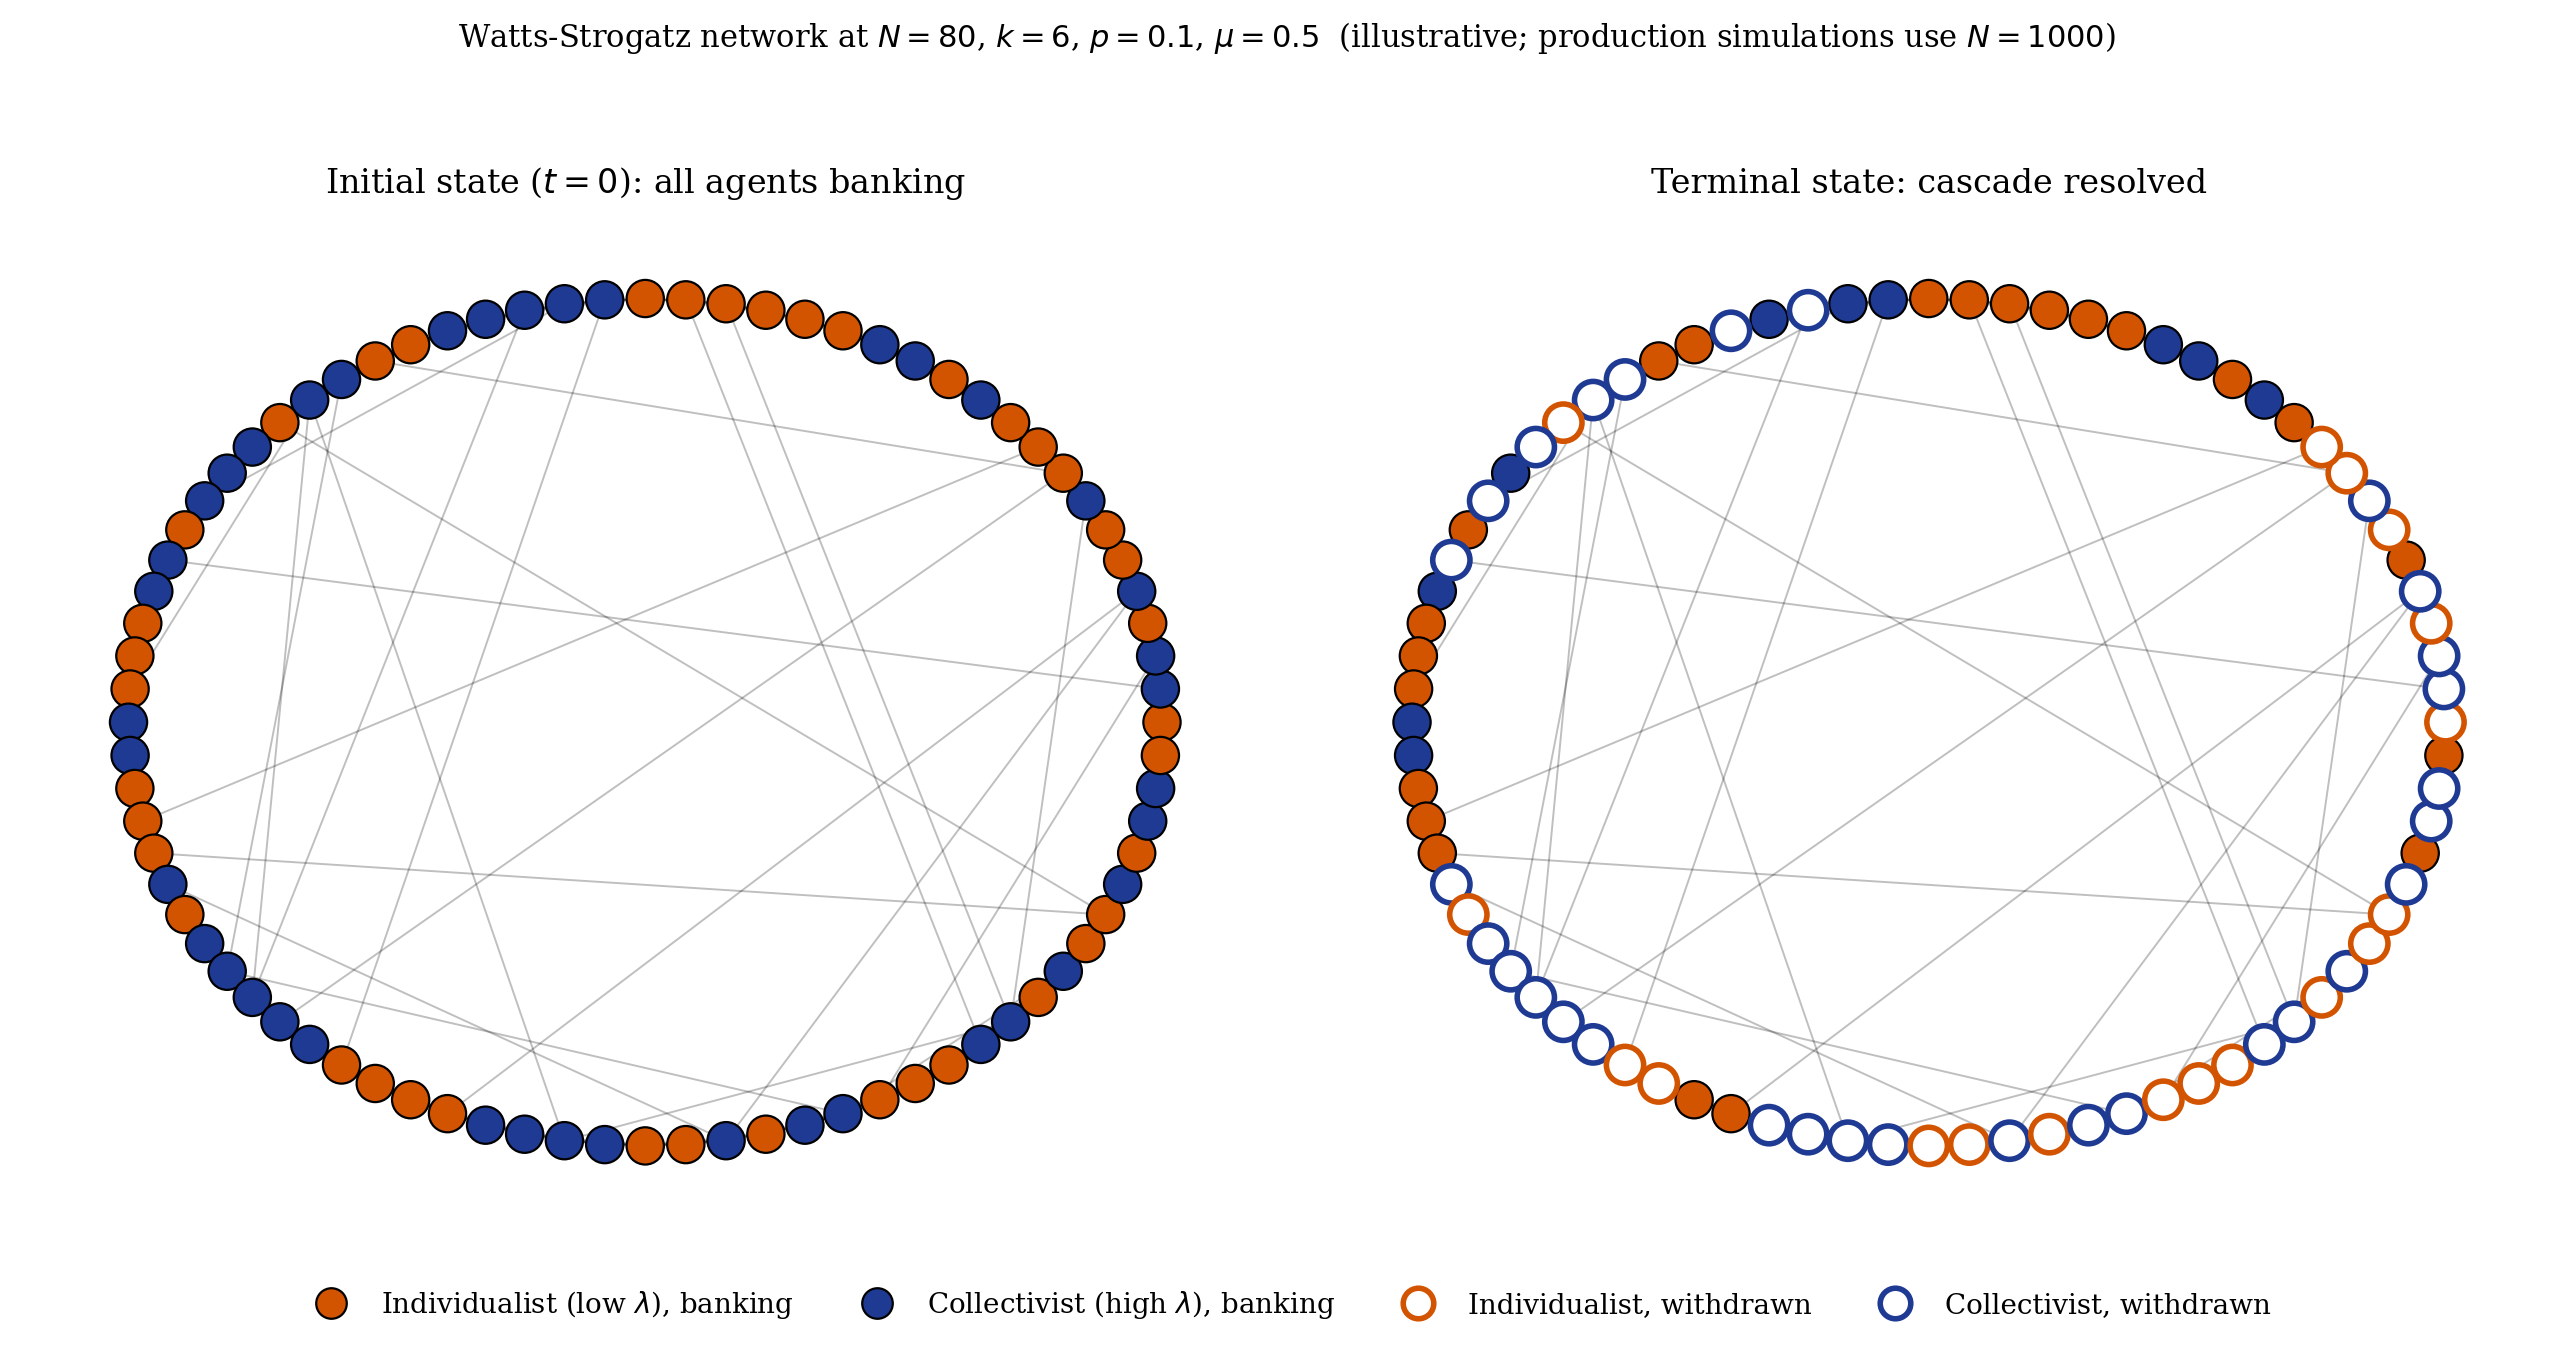
\includegraphics[width=0.9\textwidth]{figures/fig5_network_snapshot}
\caption{Pedagogical illustration of the simulation environment. Left: initial state at $t=0$, with all agents in the banked state. Each circle is one agent, positioned on a ring; arcs along the ring are local connections to nearest neighbors, and chords across the interior are long-range rewires that give the Watts-Strogatz network its small-world property. Color encodes cultural type, with individualist agents (low $\lambda$, weighting private signals) shown in orange and collectivist agents (high $\lambda$, weighting neighbor signals) shown in blue --- a heterogeneity introduced in §4. Right: terminal state of an illustrative cascade, with withdrawn agents shown as hollow markers. Each agent's color is preserved across panels so the cultural mix of the surviving banking subpopulation is visible. Figure parameters: $N=80$, $k=6$, $p=0.1$, $\mu=0.5$; production simulations use $N=1000$. The cascade pattern in the right panel is generated by a stylized recruitment rule for visual clarity rather than a full Monte Carlo simulation.}
\label{fig:network-snapshot}
\end{figure}

\textbf{Exogenous withdrawal distribution.} The number of exogenous
withdrawals at the start of each model run is drawn from a truncated
Geometric distribution:

\[W_{\text{exog}} \sim \text{Geometric}(p_g)\big|_{[0,\, 1000]}\]

with \(p_g = 0.1\) fixed. The truncated Geometric is approximately
memoryless and right-skewed, meaning most runs have few exogenous
withdrawals but the occasional run has a large exogenous shock.

\subsection{Model Event Timeline}

Each model run proceeds in two phases.

\paragraph{Phase 1: Exogenous Withdrawals}

\begin{enumerate}
\def\labelenumi{\arabic{enumi}.}
\item
  A realization \(w_{\text{exog}}\) is drawn from the truncated
  Geometric distribution.
\item
  \(w_{\text{exog}}\) agents are selected uniformly at random (without
  replacement) from the full agent population and forced to withdraw.
\item
  Each selected agent receives its payment per the payment formula
  above. The vault is decremented accordingly.
\item
  If the vault reaches zero or below after Phase 1, the model terminates
  immediately and records a bank failure.
\end{enumerate}

The exogenous shock represents withdrawal demand arising from outside
the model's social dynamics: liquidity needs, idiosyncratic shocks, or
the initial ``runners'' who set the process in motion.

\paragraph{Phase 2: Endogenous Withdrawals (Iterated)}

Phase 2 iterates over all agents still banked, in a randomly shuffled
order, until either the bank fails or no agent changes state in a full
pass (a stable equilibrium is reached).

For each agent i still banked, the following steps occur:

\textbf{Step 1: Observe network neighbors.} Agent i identifies its
network neighbors and counts how many have already withdrawn:

\[n_{\text{withdrawn}} = \#\{j \in \mathcal{N}(i) : \text{banked}_j = \text{false}\}\]
\[\hat{\pi}_{\text{withdrawn}} = \frac{n_{\text{withdrawn}}}{|\mathcal{N}(i)|}\]

\textbf{Step 2: Infer population-level withdrawals.} The agent scales
its observed neighbor withdrawal rate to estimate total withdrawals in
the full population:

\[\hat{W}_{\text{total}} = \text{round}\left(\hat{\pi}_{\text{withdrawn}} \times N\right)\]

This is a naive but tractable inference step: the agent treats its local
neighborhood as a representative sample of the population.

\textbf{Step 3: Sample possible future withdrawal totals.} Using the
observed withdrawal count as a lower bound, the agent samples D = 1,000
possible total withdrawal counts from a truncated Geometric
distribution:

\[\tilde{W}^{(k)} \sim \text{Geometric}(p_g)\big|_{[\hat{W}_{\text{total}},\, N-1]}, \quad k = 1, \ldots, D\]

This represents the agent's uncertainty about how many \emph{additional}
withdrawals might occur.

\textbf{Step 4: Monte Carlo comparison --- ``withdraw now''
vs.~``stay.''}

For each trial k = 1, \ldots, D, the agent runs two counterfactual
simulations on a cloned copy of the current model state:

\begin{itemize}
\item
  \textbf{Withdraw now scenario} (\emph{initWithdrawResults}): Agent i
  withdraws immediately from the current state of the cloned model. The
  payment received is recorded. This is compared against \(d_i\) to
  determine whether the agent received its full deposit.
\item
  \textbf{Stay and withdraw later scenario} (\emph{subModResults}): In a
  separate clone, the agent first forces all already-withdrawn neighbors
  to withdraw (reflecting observed information), then removes
  \(\tilde{W}^{(k)} - n_{\text{withdrawn}}\) additional random agents
  (reflecting anticipated future withdrawals), and \emph{then} agent i
  withdraws. The payment received is again compared against \(d_i\).
\end{itemize}

This yields two empirical probabilities:

\[\hat{P}_{\text{WD}} = \frac{1}{D} \sum_{k=1}^{D} \mathbf{1}\left[\text{payment}_{\text{now}}^{(k)} = d_i\right]\]

\[\hat{P}_{\text{stay}} = \frac{1}{D} \sum_{k=1}^{D} \mathbf{1}\left[\text{payment}_{\text{later}}^{(k)} = d_i\right]\]

\textbf{Step 5: Decision.} Agent i withdraws if:

\[\hat{P}_{\text{WD}} > \hat{P}_{\text{stay}}\]

That is, the agent withdraws if it is more likely to receive its full
deposit by withdrawing \emph{now} than by waiting. If the agent
withdraws, the halt flag is reset (Phase 2 continues for another pass);
if no agent withdraws in a full pass, Phase 2 terminates with no bank
failure.

\paragraph{Termination}

The run terminates under one of two conditions: 1. \textbf{Bank
failure}: the vault reaches zero or below at any point in either phase.
Result recorded: failure (= 1). 2. \textbf{Stability}: a full pass
through all banked agents in Phase 2 completes with no agent
withdrawing. Result recorded: no failure (= 0).

\begin{center}\rule{0.5\linewidth}{0.5pt}\end{center}

\section{Cultural Heterogeneity: Individualism and Collectivism}
\label{sec:abm_culture}

\subsection{Motivation}

The base model treats all agents identically in their decision-making:
each agent observes the same neighbor signal type, infers
population-level withdrawals the same way, and applies the same Monte
Carlo comparison. In reality, depositors vary in how much they rely on
social signals versus their own independent assessment. The 2023 SVB
collapse illustrates this: some depositors acted on social media signals
within hours, while others waited for independent confirmation. This
heterogeneity in susceptibility to social influence is a first-order
feature of real bank runs.

The extension introduces a continuous \textbf{individualism parameter} $\lambda$
$\in$ {[}0, 1{]} for each agent, representing the weight placed on the
neighbor signal versus the agent's own Monte Carlo prior when forming
beliefs about total population withdrawals. The parameter is not
assigned arbitrarily --- it emerges from a cultural formation process on
the same network used in the bank-run simulation.

\subsection{Cultural Formation: Flache-Macy Warm-Up}

Before the bank-run simulation begins, agents undergo a cultural warm-up
phase based on the Flache \& Macy (2011) social influence model with
negative influence. Each agent holds opinions on F = 5 cultural
dimensions, each in {[}$-$1, 1{]}, initialised uniformly at random.

At each warm-up tick, agents interact with a random network neighbour:

\begin{enumerate}
\def\labelenumi{\arabic{enumi}.}
\item
  \textbf{Influence weight:}
  \(w_{ij} = \frac{1}{F} \sum_f a_{if} \cdot a_{jf} \in [-1, 1]\).
  Positive for culturally similar dyads (correlated opinion profiles),
  negative for dissimilar (anti-correlated).
\item
  \textbf{Opinion update:}
  \(\Delta a_{if} = \alpha \cdot w_{ij} \cdot (a_{jf} - a_{if})\),
  clamped to {[}$-$1, 1{]}. The learning rate $\alpha$ (\texttt{warmupAlpha}) is
  a swept parameter.

  \begin{itemize}
  \item
    \(w_{ij} > 0\): agent moves \textbf{toward} neighbour (cultural
    convergence). \texttt{adoptCount} increments.
  \item
    \(w_{ij} \leq 0\): agent moves \textbf{away} from neighbour
    (cultural repulsion). \texttt{resistCount} increments.
  \end{itemize}
\end{enumerate}

The dynamics produce cultural polarisation: agents in homogeneous
network clusters converge to shared extreme opinions, while agents at
cluster boundaries are pulled in opposing directions. Convergence occurs
when all opinions reach $\pm$1 extremes.

After convergence, the warm-up produces a \textbf{cultural resistance
score} for each agent:

\[\lambda_i^{\text{warmup}} = \frac{\text{resistCount}_i}{\text{adoptCount}_i + \text{resistCount}_i}\]

Agents embedded deep within a cultural cluster accumulate high
adoptCount $\to$ low \(\lambda^{\text{warmup}}\) (culturally conformist).
Agents at cluster boundaries accumulate high resistCount $\to$ high
\(\lambda^{\text{warmup}}\) (culturally resistant). This score reflects
the agent's structural position in the network's cultural landscape.

\subsection{Two-Type Assignment and $\lambda$ Draws}

The warm-up resistance scores create a ranking of agents. The parameter
$\mu$ (\texttt{fracIndividualists}) sets the cutoff: the top $\mu$ fraction by
warm-up \(\lambda^{\text{warmup}}\) is labeled \textbf{type I}
(individualist); the remainder is labeled \textbf{type C}
(collectivist). The warm-up determines \emph{who} gets assigned to which
type; $\mu$ controls \emph{how many}.

Each agent then draws a continuous $\lambda$ from a Beta distribution centred on
their type mean, with shared concentration $\kappa$ = 20:

\begin{itemize}
\item
  \textbf{Type I:}
  \(\lambda \sim \text{Beta}(\lambda_I \cdot \kappa,\ (1 - \lambda_I) \cdot \kappa)\),
  with \(E[\lambda] = \lambda_I\)
\item
  \textbf{Type C:}
  \(\lambda \sim \text{Beta}(\lambda_C \cdot \kappa,\ (1 - \lambda_C) \cdot \kappa)\),
  with \(E[\lambda] = \lambda_C\)
\end{itemize}

The swept parameters \(\lambda_I\) and \(\lambda_C\) are constrained so
that \(\lambda_I < \lambda_C\) (individualists are less susceptible to
social signals than collectivists). At $\kappa$ = 20, the Beta distributions
are tightly peaked ($\sigma$ $\approx$ 0.09 at a mean of 0.5), providing within-type
heterogeneity without overlap between types.

Note that if \(\lambda_I = \lambda_C\), the two Beta distributions are
identical, the type labels become meaningless, and $\mu$ has no effect. The
entire mechanism collapses to a homogeneous population with a single
shared signal weight.

\subsection{Modified Belief Formation in Phase 2}

The agent's drawn $\lambda$ enters the endogenous decision-making phase (Phase
2) through a modified belief formation step. Where the base model drew
future withdrawal estimates from a truncated Geometric conditioned on
the observed count, the extended model blends two information sources:

\begin{enumerate}
\def\labelenumi{\arabic{enumi}.}
\item
  \textbf{Own MC prior:} D = 1,000 draws from the untruncated
  Geometric(0.1) distribution --- the agent's independent estimate of
  total population withdrawals, uninformed by local observation.
\item
  \textbf{Neighbor signal:} The point estimate
  \(\hat{W}_{\text{total}} = \text{round}(\hat{\pi}_{\text{withdrawn}} \times N)\)
  from observing network neighbors.
\end{enumerate}

For each Monte Carlo trial k:

\[\text{blendedTotal}_k = \text{round}\left((1 - \lambda) \cdot \text{mcDraw}_k + \lambda \cdot \hat{W}_{\text{total}}\right)\]

\[\text{additionalWithdrawals}_k = \max(0,\ \text{blendedTotal}_k - n_{\text{withdrawn}})\]

The agent's $\lambda$ interpolates between two extremes: - \textbf{$\lambda$ near 0
(individualist):} Blended estimate $\approx$ mcDraw. The agent ignores what its
neighbors are doing and relies on its own prior. Self-reliant; withdraws
only when its independent estimate of risk is high. - \textbf{$\lambda$ near 1
(collectivist):} Blended estimate $\approx$ \(\hat{W}_{\text{total}}\). The
agent follows the neighbor signal and ignores its own prior.
Signal-driven; easily tipped by observed withdrawal activity.

The rest of Phase 2 proceeds as in the base model: the agent runs D
Monte Carlo trials comparing ``withdraw now'' versus ``stay,'' using the
blended additional withdrawal counts, and withdraws if P(full deposit
\textbar{} withdraw now) \textgreater{} P(full deposit \textbar{} stay).

Importantly, $\lambda$ plays no role in Phase 1 (exogenous withdrawals), which
remains purely random.

\subsection{Theoretical Predictions}

\paragraph{Prediction 1: More individualists $\to$ higher bank-run probability (first-order effect)}

The untruncated Geometric(0.1) prior has a mean of approximately 9.
After a typical small exogenous shock (say 2--3 withdrawals out of 1,000
agents), the neighbor signal for most agents is low. Collectivists blend
heavily toward that low neighbor signal, estimate low risk, and stay.
Individualists largely ignore the low neighbor signal and draw from
their Geometric prior, estimating approximately 9 withdrawals on average
--- perceiving more risk than actually exists.

The first-order prediction is therefore monotonic: \textbf{increasing $\mu$
(more individualists) increases bank-run probability}, because
individualists are more trigger-happy. Their MC prior is uncorrelated
with actual conditions and systematically overestimates withdrawal
counts relative to the neighbor signal after a typical small shock.

\paragraph{Prediction 2: Non-monotonicity at intermediate $\mu$ (second-order interaction effect)}

The interaction between types may produce a bank-run probability that
peaks at intermediate $\mu$ rather than at $\mu$ = 1. The mechanism:

\begin{itemize}
\item
  At \textbf{$\mu$ = 0} (all collectivist): the herd stays calm because the
  herd sees calm. If the exogenous shock is small, the neighbor signal
  is low, and nobody panics. But if the shock exceeds a critical mass,
  the entire population cascades.
\item
  At \textbf{$\mu$ = 1} (all individualist): agents ignore each other. Some
  withdraw due to high MC draws, but there is no amplification --- noise
  doesn't cascade.
\item
  At \textbf{intermediate $\mu$}: individualists produce ``noise''
  withdrawals driven by tail draws from their Geometric prior. Those
  withdrawals are picked up as genuine signal by the remaining
  collectivists, who amplify them through the neighbor channel. The
  collectivists then trigger further withdrawals, which feed back into
  other collectivists' signals. The result is a cascade that
  \emph{neither} an all-collectivist nor all-individualist population
  would have produced.
\end{itemize}

The fixed-point equations for withdrawal thresholds capture this
coupling:

\[s^*_I = \theta - \lambda_I \cdot f\bigl(\mu \cdot \Phi(s^*_I) + (1-\mu) \cdot \Phi(s^*_C)\bigr)\]
\[s^*_C = \theta - \lambda_C \cdot f\bigl(\mu \cdot \Phi(s^*_I) + (1-\mu) \cdot \Phi(s^*_C)\bigr)\]

The aggregate signal fed back into everyone's decision is a weighted mix
of both types' behavior. Because $\lambda_I$ $\ne$ $\lambda_C$, this system does not
reduce to a simple monotone function of $\mu$.

\paragraph{Prediction 3: The $\lambda$ gap amplifies the interaction effect}

\begin{itemize}
\item
  \textbf{Large gap} (e.g., $\lambda_I$ = 0.1, $\lambda_C$ = 0.9): Types behave very
  differently --- individualists are nearly immune to social signal,
  collectivists are nearly pure herd followers. The noise-amplification
  mechanism is strongest; any non-monotonicity in $\mu$ should be most
  pronounced.
\item
  \textbf{Small gap} (e.g., $\lambda_I$ = 0.3, $\lambda_C$ = 0.5): Types are more
  similar. $\mu$ matters less. The bank-run probability curve across $\mu$
  should be flatter.
\item
  \textbf{Zero gap} ($\lambda_I$ = $\lambda_C$): No type distinction. $\mu$ has no effect.
  The mechanism is absent.
\end{itemize}

\paragraph{Prediction 4: warmupAlpha affects type assignment quality}

The learning rate $\alpha$ does not change the bank-run mechanism directly but
changes \emph{who} ends up in each type:

\begin{itemize}
\item
  \textbf{Low $\alpha$} $\to$ slow cultural convergence $\to$ more agents remain in
  ambiguous boundary positions $\to$ the warm-up ranking is noisier $\to$ type
  assignment is less correlated with network structure.
\item
  \textbf{High $\alpha$} $\to$ fast convergence to sharp cultural clusters $\to$ clear
  separation between cluster-interior agents (collectivist) and boundary
  agents (individualist) $\to$ type assignment reflects network topology
  more faithfully.
\end{itemize}

\paragraph{Prediction 5: Network-culture correlation}

Because the warm-up and bank-run share the same Watts-Strogatz network,
there is an endogenous correlation between network position and cultural
type:

\begin{itemize}
\item
  \textbf{Cluster-interior agents} (many similar neighbors in warm-up)
  accumulate high adoptCount $\to$ low warm-up $\lambda$ $\to$ labeled collectivist.
  These same agents tend to be well-connected nodes who observe many
  neighbors during Phase 2.
\item
  \textbf{Boundary agents} (neighbors from different cultural clusters)
  accumulate high resistCount $\to$ high warm-up $\lambda$ $\to$ labeled individualist.
  These tend to be structural bridges with fewer same-cluster
  connections.
\end{itemize}

Collectivists are therefore disproportionately high-degree,
well-embedded nodes --- exactly the agents who receive the strongest
social signal during Phase 2. Individualists sit at the network
periphery where they observe less. This structural correlation means
that it is not only the \emph{fraction} of each type but \emph{where}
each type sits in the network that matters for cascade dynamics.

\paragraph{Prediction 6: Interactions with baseline parameters}

The cultural heterogeneity mechanism should interact with the original
model parameters:

\begin{itemize}
\item
  \textbf{Reserve ratio:} Higher reserves make the bank harder to fail,
  potentially muting the non-monotonicity in $\mu$ --- there is less room
  for cascade regardless of cultural composition.
\item
  \textbf{Network connectivity (k):} Higher k means more neighbors
  observed, which amplifies the collectivist channel. The
  non-monotonicity in $\mu$ may be stronger on denser networks.
\item
  \textbf{Deposit heterogeneity ($\sigma$):} Heavier-tailed deposit
  distributions create large depositors with more at stake. If large
  depositors happen to be collectivist (cluster-interior,
  well-connected), their signal-driven withdrawals deplete the vault
  disproportionately fast.
\end{itemize}

\begin{center}\rule{0.5\linewidth}{0.5pt}\end{center}

\section{Simulation Design}
\label{sec:abm_design}

\subsection{Parameter Space}

The model is run across a full factorial sweep of the following
parameters:

\begin{longtable}[]{@{}ll@{}}
\toprule\noalign{}
Parameter & Values \\
\midrule\noalign{}
\endhead
\bottomrule\noalign{}
\endlastfoot
Reserve ratio (r) & 0.2, 0.4 \\
Deposit insurance quantile (q) & 0.1, 0.2, 0.3, 0.4 \\
LogNormal $\sigma$ (deposit heterogeneity) & 2.0, 3.0 \\
Watts-Strogatz k (mean degree) & 6, 10, 50 \\
Watts-Strogatz p (rewiring probability) & 0.05, 0.15 \\
Warm-up learning rate ($\alpha$) & 0.1, 0.3, 0.5 \\
Fraction individualists ($\mu$) & 0.0, 0.25, 0.5, 0.75, 1.0 \\
Individualist signal weight mean ($\lambda_I$) & 0.1, 0.2, 0.3 \\
Collectivist signal weight mean ($\lambda_C$) & 0.5, 0.7, 0.9 \\
\end{longtable}

The LogNormal mean parameter $\mu_{LN}$ is fixed at 1.0. The exogenous
withdrawal probability \(p_g\) is fixed at 0.1. The agent count N is
fixed at 1,000. The Monte Carlo depth D is fixed at 1,000 trials per
agent per decision. The warm-up uses F = 5 cultural dimensions, a
maximum of 500 ticks, and convergence threshold $\epsilon$ = 1e-6. The
within-type Beta concentration is $\kappa$ = 20.

The $\lambda_I$ and $\lambda_C$ ranges are non-overlapping (max $\lambda_I$ = 0.3 \textless{}
min $\lambda_C$ = 0.5), ensuring that $\lambda_I$ \textless{} $\lambda_C$ holds for every
combination.

This yields 2 $\times$ 4 $\times$ 2 $\times$ 3 $\times$ 2 $\times$ 3 $\times$ 5 $\times$ 3 $\times$ 3 = 12,960 distinct
parameter combinations. Each combination is run with 5 distinct random
seeds for model initialization (controlling agent deposit draws, network
construction, and warm-up dynamics), and each seed is replicated 10
times (controlling the stochastic sequence of withdrawals and agent
ordering within a run). This gives 50 runs per parameter combination and
648,000 total runs.

\subsection{Distributed Execution}

Runs are distributed via SLURM on an HPC cluster. Each of the 12,960
parameter combinations is submitted as an independent SLURM array task,
with at most 50 tasks running concurrently. Each task launches a Julia
process with 16 cores (1 master + 15 workers). Each task writes to an
isolated output directory (\texttt{task\_\{id\}/}) to avoid filename
collisions across tasks. Within each task, the 50 runs (5 seeds $\times$ 10
iterations) are distributed across the 15 worker processes via a locked
work-queue pattern.

\subsection{Experiment Structure}

The parameter sweep is analyzed as a set of structured experiments, each
isolating the effect of one or two parameters while holding others at
reference values or examining the full cross. The baseline parameters
(reserve ratio, deposit insurance, $\sigma$, k, p) are analyzed first to
confirm directional consistency with the 96-combination base model. The
cultural heterogeneity parameters ($\alpha$, $\mu$, $\lambda_I$, $\lambda_C$) are then examined
for their marginal and interaction effects on bank-run probability.

\begin{center}\rule{0.5\linewidth}{0.5pt}\end{center}

\section{Simulation Results}
\label{sec:abm_results}

\subsection{Output Variables}

Each run produces the following outputs, written to CSV files in the
data directory:

\textbf{\texttt{bankRunResults\{core\}.csv}} --- primary outcome file.
One row per run.

\begin{longtable}[]{@{}ll@{}}
\toprule\noalign{}
Column & Description \\
\midrule\noalign{}
\endhead
\bottomrule\noalign{}
\endlastfoot
\texttt{key} & Unique run identifier (timestamp + seeds) \\
\texttt{result} & Binary: 1 = bank failure (vault exhausted), 0 =
stable \\
\end{longtable}

\textbf{\texttt{bankRunExogenous\{core\}.csv}} --- one row per exogenous
withdrawal event.

\begin{longtable}[]{@{}ll@{}}
\toprule\noalign{}
Column & Description \\
\midrule\noalign{}
\endhead
\bottomrule\noalign{}
\endlastfoot
\texttt{key} & Run identifier \\
\texttt{agent} & Agent index \\
\texttt{exogenous} & Always \texttt{true} in this file \\
\texttt{deposit} & Agent's deposit amount \\
\texttt{tick} & Always 0 (Phase 1) \\
\texttt{vault} & Vault level after this withdrawal \\
\end{longtable}

\textbf{\texttt{bankRunEndogenous\{core\}.csv}} --- one row per agent
decision in Phase 2 (including agents that decide \emph{not} to
withdraw).

\begin{longtable}[]{@{}
  >{\raggedright\arraybackslash}p{(\linewidth - 2\tabcolsep) * \real{0.5000}}
  >{\raggedright\arraybackslash}p{(\linewidth - 2\tabcolsep) * \real{0.5000}}@{}}
\toprule\noalign{}
\begin{minipage}[b]{\linewidth}\raggedright
Column
\end{minipage} & \begin{minipage}[b]{\linewidth}\raggedright
Description
\end{minipage} \\
\midrule\noalign{}
\endhead
\bottomrule\noalign{}
\endlastfoot
\texttt{key} & Run identifier \\
\texttt{agent} & Agent index \\
\texttt{withdraw} & Boolean: did the agent withdraw? \\
\texttt{deposit} & Agent's deposit amount \\
\texttt{tick} & Phase 2 iteration number \\
\texttt{vault} & Vault level at time of decision \\
\texttt{wdProb} & \(\hat{P}_{\text{WD}}\): estimated P(full deposit
\textbar{} withdraw now) \\
\texttt{stayProb} & \(\hat{P}_{\text{stay}}\): estimated P(full deposit
\textbar{} stay) \\
\end{longtable}

\textbf{\texttt{agents\{core\}.csv}} --- one row per agent per run.

\begin{longtable}[]{@{}
  >{\raggedright\arraybackslash}p{(\linewidth - 2\tabcolsep) * \real{0.5000}}
  >{\raggedright\arraybackslash}p{(\linewidth - 2\tabcolsep) * \real{0.5000}}@{}}
\toprule\noalign{}
\begin{minipage}[b]{\linewidth}\raggedright
Column
\end{minipage} & \begin{minipage}[b]{\linewidth}\raggedright
Description
\end{minipage} \\
\midrule\noalign{}
\endhead
\bottomrule\noalign{}
\endlastfoot
\texttt{key} & Run identifier \\
\texttt{idx} & Agent index \\
\texttt{deposit} & Agent deposit amount \\
\texttt{individualism} & Agent's drawn $\lambda$ (from Beta distribution, used
in Phase 2 blending) \\
\texttt{warmupLambda} & Raw warm-up resistance score (used only for type
ranking) \\
\texttt{agentType} & ``I'' (individualist) or ``C'' (collectivist) \\
\end{longtable}

\textbf{\texttt{bankRunParametersInit.csv}} --- one row per run,
parameter values.

\begin{longtable}[]{@{}ll@{}}
\toprule\noalign{}
Column & Description \\
\midrule\noalign{}
\endhead
\bottomrule\noalign{}
\endlastfoot
\texttt{seed1} & Initialization seed (controls deposits and network) \\
\texttt{iteration} & Within-seed replication index \\
\texttt{graphParams1} & Watts-Strogatz k \\
\texttt{graphParams2} & Watts-Strogatz p \\
\texttt{reserveRatio} & Reserve ratio r \\
\texttt{depositInsuranceQuantile} & Insurance quantile q \\
\texttt{warmupAlpha} & Flache-Macy learning rate $\alpha$ \\
\texttt{fracIndividualists} & Fraction type I ($\mu$) \\
\texttt{lambdaI} & Individualist signal weight mean \\
\texttt{lambdaC} & Collectivist signal weight mean \\
\texttt{seed2} & Run-level stochastic seed \\
\texttt{key} & Run identifier \\
\end{longtable}

\subsection{Experiment 1: Effect of Reserve Ratio}

This experiment compares bank-failure rates between the two
reserve-ratio levels (r = 0.2 and r = 0.4) pooled across all other
parameters. The predicted direction follows directly from Theorem 2
(§9.6): higher reserve ratios increase the per-agent survival
probability p\_S($\tau$, C, N, q) by raising C, and the expected
endogenous-cascade size is therefore weakly decreasing in r. The
empirical question is whether the magnitude of this effect is large
enough to dominate the cultural and network channels, or whether
sufficient network connectivity and cultural composition can produce
runs even at r = 0.4. Quantitative results pending sweep completion.

\subsection{Experiment 2: Effect of Deposit Insurance}

This experiment varies the deposit-insurance quantile q across \{0.1,
0.2, 0.3, 0.4\}, holding the reserve ratio fixed. Because the insurance
cap is the q-th quantile of the log-normal deposit distribution, higher
q both raises the absolute insured amount and shifts the mass of fully
insured agents upward. The predicted direction is decreasing run
probability in q, with potential non-linearity at low coverage levels
where small additions to the cap insure many additional small
depositors. A secondary diagnostic is the distribution of estimated
wdProb and stayProb values across insurance levels: under the Monte
Carlo decision rule, higher insurance should compress the gap between
these two probabilities for small depositors and leave it unaffected for
large ones. Quantitative results pending sweep completion.

\subsection{Experiment 3: Effect of Deposit Heterogeneity}

This experiment compares bank-failure rates between $\sigma$ = 2.0 and $\sigma$ = 3.0
in the log-normal deposit distribution. Higher $\sigma$ produces a heavier tail
and concentrates more total deposit mass in the largest agents, which in
the model are also the agents whose individual withdrawal can deplete
the vault disproportionately. The predicted direction is increasing run
probability in $\sigma$, with an interaction effect: high-$\sigma$ regimes should also
show greater sensitivity to network position effects, because the
largest depositors' network embeddedness becomes a first-order driver of
cascade dynamics. The diagnostic plot is the distribution of vault
depletion (as a fraction of initial vault) attributable to the top
decile of depositors across $\sigma$ regimes. Quantitative results pending
sweep completion.

\subsection{Experiment 4: Effect of Network Structure}

This experiment examines bank-failure rates across the Watts-Strogatz k
$\times$ p factorial, holding cultural and baseline parameters fixed. The
predicted direction is increasing run probability in k (more observed
neighbors strengthen the social-signal channel) and ambiguous in p
(random rewiring can either accelerate cascades by creating long-range
bridges or dilute local clustering and reduce coordination among similar
agents). The interaction with cultural composition is critical: the k $\times$
$\mu$ interaction surface should reveal whether dense networks (k = 50)
amplify the cultural-heterogeneity effects through the collectivist
herding channel. Quantitative results pending sweep completion.

\subsection{Experiment 5: Effect of Cultural Composition ($\mu$)}

This experiment is the central test of the chapter's theoretical
contribution. Bank-failure probability is computed as a function of $\mu$ $\in$
\{0.0, 0.25, 0.5, 0.75, 1.0\}, stratified by the signal-weighting gap
$\lambda_C$ $-$ $\lambda_I$ and by reserve ratio. The theory chapter (Chapter 1, §4.6)
separates the cultural-composition prediction into two distinct
channels: P6a, a direct effect under which run probability is
monotonically decreasing in $\mu$ as cascade-vulnerable collectivist agents
are replaced by self-reliant individualists; and P6b, an indirect
amplification effect under which intermediate $\mu$ produces an interior
peak above the P6a baseline as individualist tail-draws seed cascades
that collectivists then amplify. The two channels share a common
amplification mechanism --- the gap $\lambda_C$ $-$ $\lambda_I$ --- but operate in
different parameter regimes and produce distinct empirical signatures.

\textbf{Provisional results (533,945 outcome-bearing simulations across
2,160 parameter cells; 47,940 simulations completed without emitting a
terminal outcome record and are excluded from rate calculations; 25
cells were still running at the time of analysis).}

The empirical pattern strongly confirms P6a. Bank-run probability is
monotonically decreasing in $\mu$, falling from 84.4\% at $\mu$ = 0 (all
collectivists) to 68.4\% at $\mu$ = 1 (all individualists) --- a
16.0-percentage-point reduction in aggregate fragility from cultural
composition alone. The decline is steepest in the interior ($\mu$ = 0.25 $\to$
0.75 produces a 10.6 pp drop) and flatter at the boundaries. Figure 1
displays the headline pattern.

\begin{figure}[t]
\centering
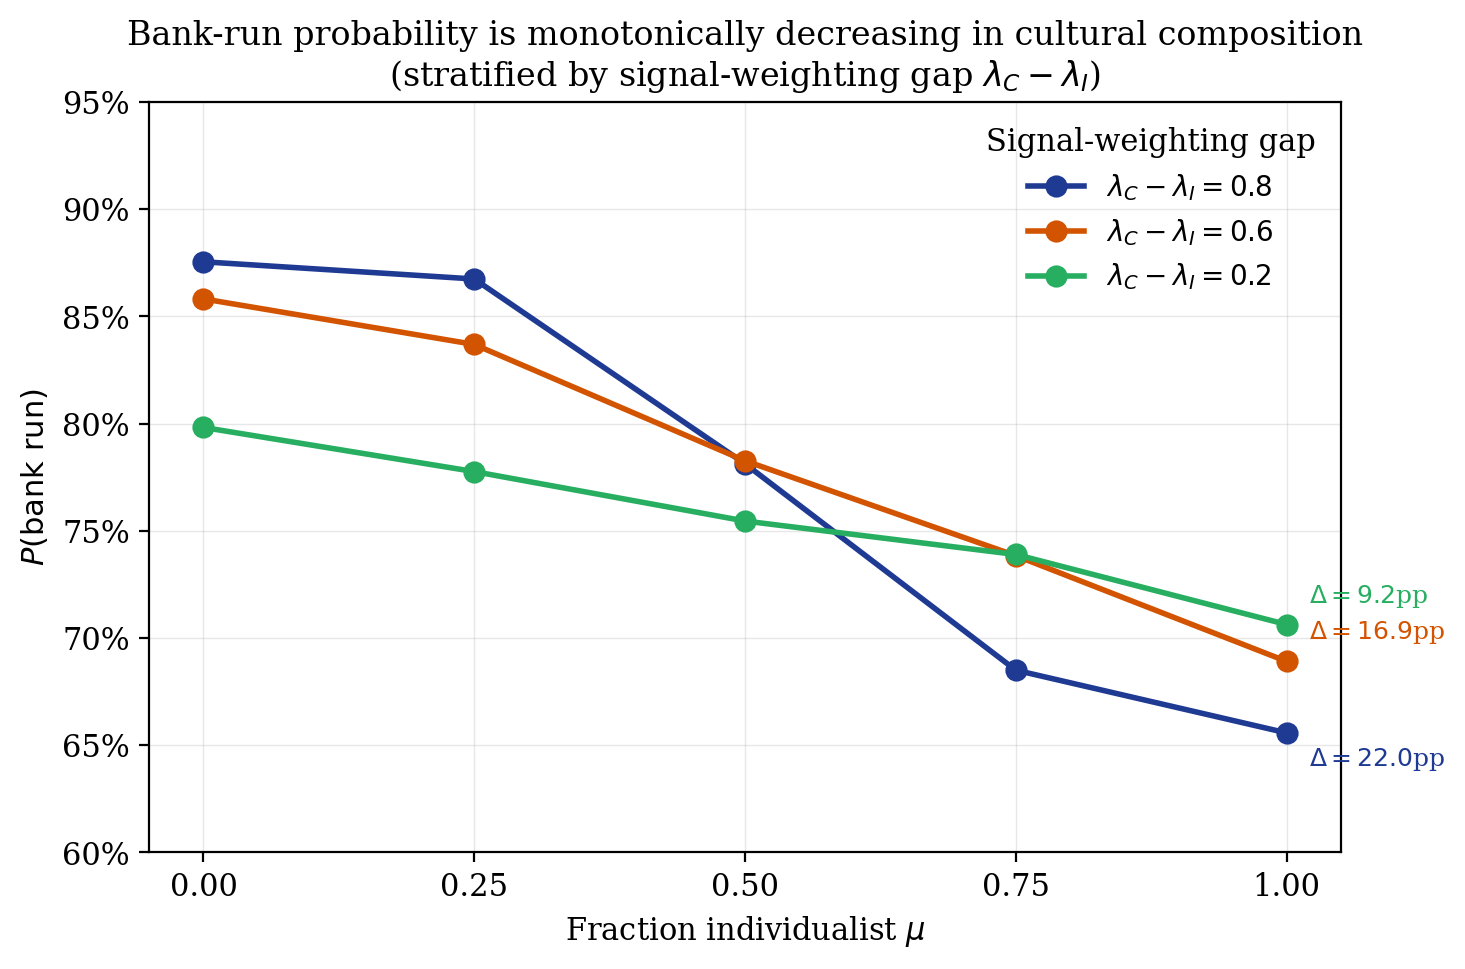
\includegraphics[width=0.85\textwidth]{figures/fig1_p6a_headline}
\caption{Bank-run probability is monotonically decreasing in the individualist population share $\mu$ (P6a confirmation), with the slope amplified by the signal-weighting gap $\lambda_C - \lambda_I$. Each line aggregates across 80--90 thousand outcome-bearing simulations per $\mu$ level. Annotations report the total decline from $\mu = 0$ to $\mu = 1$ in percentage points.}
\label{fig:p6a-headline}
\end{figure}

The $\lambda$-gap stratification supports the gap-amplification claim shared by
P6a and P6b. The decline in run probability from $\mu$ = 0 to $\mu$ = 1 is 22.0
pp at the largest gap ($\lambda_I$ = 0.1, $\lambda_C$ = 0.9), 16.9 pp at the
intermediate gap ($\lambda_I$ = 0.2, $\lambda_C$ = 0.8), and 9.2 pp at the smallest
gap ($\lambda_I$ = 0.3, $\lambda_C$ = 0.5). A wider gap between individualist
self-reliance and collectivist herding amplifies the population-share
effect: when individualists weight private signals strongly and
collectivists weight neighbor signals strongly, the composition of the
population matters most. When the two types behave similarly (small
gap), the composition matters less. The relationship is approximately
linear in the gap.

The reserve-ratio interaction is approximately null in the swept range r
$\in$ \{0.05, 0.15\}. Failure rates differ by less than 3 pp between the two
reserve levels at every value of $\mu$ --- see Figure 2. This null is
informative rather than disappointing: it confirms that the swept regime
is in the cascade-pressure-saturated zone in which the indirect P6b
channel is suppressed, since neither additional reserves nor a marginal
change in the cultural mix can shift outcomes by much. The
cultural-composition channel of P6a operates as a direct substitution
effect on the cascade-vulnerable subpopulation rather than as a
marginal-buffer effect on the bank's solvency state.

\begin{figure}[t]
\centering
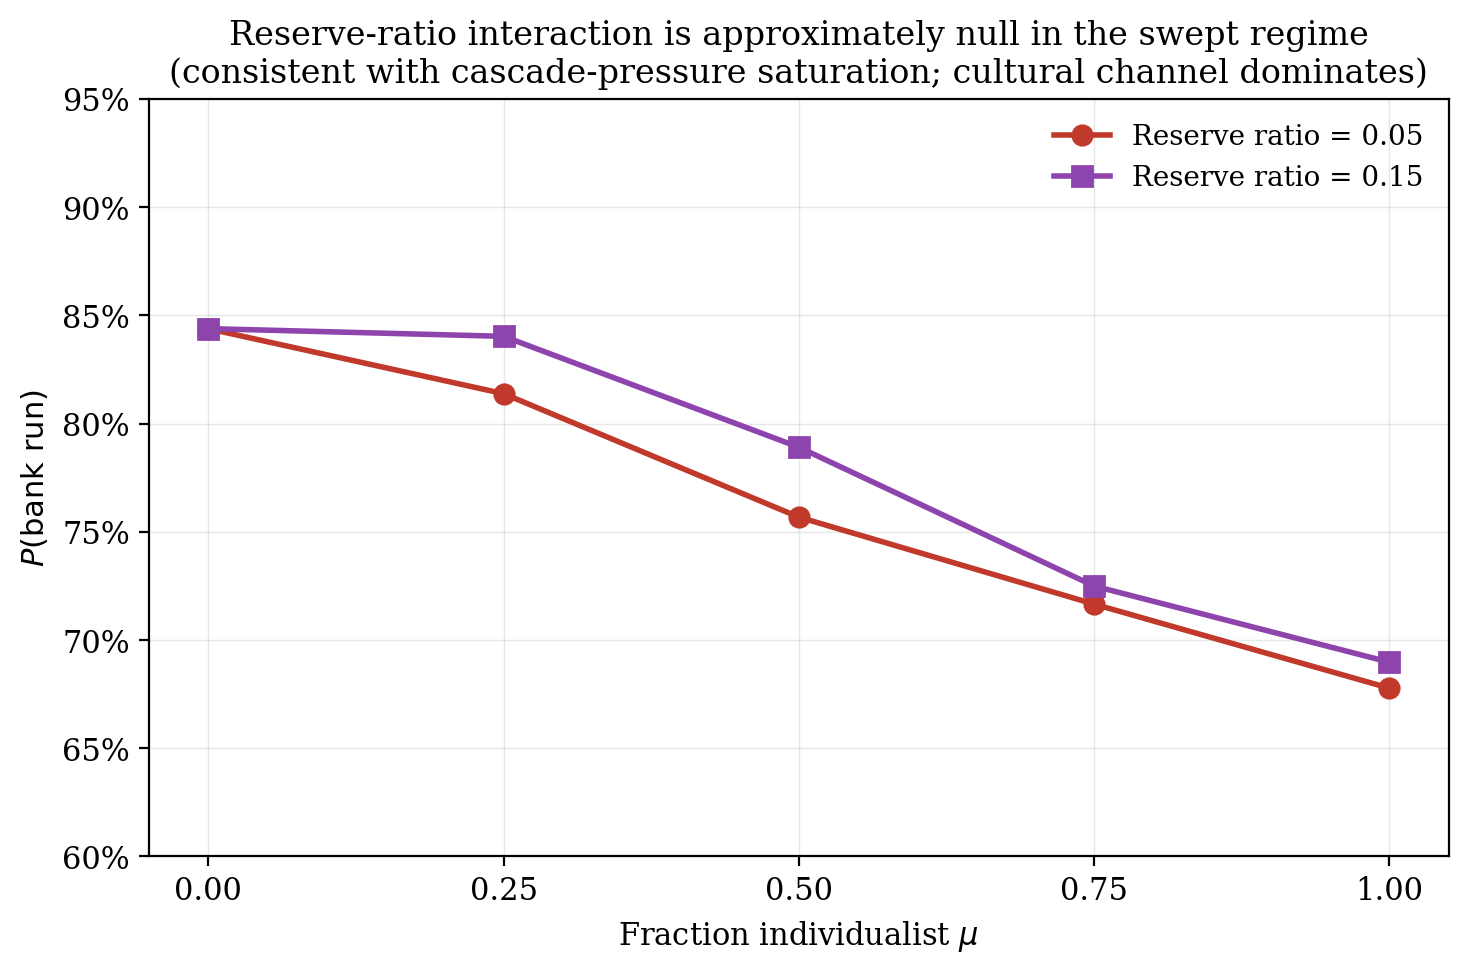
\includegraphics[width=0.85\textwidth]{figures/fig2_reserve_null}
\caption{The reserve-ratio interaction with $\mu$ is approximately null in the swept regime, with both reserve levels producing nearly coincident curves. The null supports the interpretation that the cultural-composition channel dominates the reserve channel under the parameter values used in the current sweep, and that the system is in the cascade-pressure-saturated region in which the P6b indirect channel is suppressed.}
\label{fig:reserve-null}
\end{figure}

The current sweep does not refute P6b but cannot test it. P6b's
empirical signature --- a residual interior hump in run probability
above the P6a baseline --- is observable only when cascade pressure is
intermediate, that is, when the regime is neither so aggressive that
runs occur near-universally regardless of cultural composition nor so
mild that runs occur near-never. The current parameter region (r $\in$
\{0.05, 0.15\}, with the calibrated exogenous-withdrawal intensity used
in the production sweep) places the system squarely in the
aggressive-pressure regime: pooled failure rates exceed 65\% at every $\mu$
level, and the reserve null indicates that the system has limited
marginal sensitivity to small changes in the buffer parameters. In such
a regime the indirect P6b channel is saturated and observationally
indistinguishable from the direct P6a channel --- both produce monotonic
declines, the indirect channel because the interior peak it would
otherwise generate is censored above by the saturation ceiling. A
follow-on sweep at higher reserve ratios (r $\ge$ 0.2) and lower
exogenous-withdrawal intensity is therefore required to test P6b
cleanly; this is identified as the principal direction for future
computational work in §7.

Together, these results establish that cultural composition is a
first-order driver of run dynamics in the agent-based model, with effect
magnitude (16.0 pp on aggregate fragility, 22.0 pp at the maximum
signal-weighting gap) comparable to or exceeding the reserve-ratio
variation in the same sweep. The direction of the effect --- more
individualists implies fewer aggregate runs --- appears, on first
reading, to run counter to the empirical Chapter 2 finding that
individualists exit earlier on private signals during the Celsius
collapse. The reconciliation is that the empirical chapter measures
individual exit behavior conditional on a run occurring, while the
simulation measures aggregate run probability conditional on cultural
composition. Individualist agents in this ABM are simultaneously more
likely to exit early on private information \emph{and} more likely to
refuse to participate in herd-driven cascades late in the dynamics; the
two effects act in opposite directions on aggregate run probability,
with the latter dominating the former in the parameter region swept. The
Celsius empirical patterns and the ABM aggregate patterns are therefore
complementary rather than contradictory: the empirical chapter
identifies the individual-decision channel, the agent-based chapter
identifies the population-level consequence, and the apparent
direction-flip reflects the well-known distinction between conditional
and marginal effects in heterogeneous-agent systems.

\subsection{Experiment 6: Effect of $\lambda_I$ and $\lambda_C$}

This experiment varies the type-mean signal-weighting parameters $\lambda_I$ $\in$
\{0.1, 0.2, 0.3\} and $\lambda_C$ $\in$ \{0.5, 0.7, 0.9\} both independently (at
fixed $\mu$) and jointly. Two predictions structure the analysis: (i) at
fixed $\mu$, increasing $\lambda_C$ (making collectivists more herd-driven) should
raise run probability through the amplification channel, with the
magnitude of the effect modulated by $\mu$ --- collectivists matter more
when there are more of them; and (ii) decreasing $\lambda_I$ (making
individualists more self-reliant) has an ambiguous net effect --- it can
either suppress noise withdrawals (because individualists become less
reactive to anything) or fail to suppress them (because the Geometric
prior dominates either way). The interaction surface of $\lambda_I$ $\times$ $\lambda_C$ $\times$ $\mu$
is the primary diagnostic. Quantitative results pending sweep
completion.

\subsection{Experiment 7: Effect of Warm-Up Learning Rate ($\alpha$)}

This experiment varies the Flache-Macy learning rate $\alpha$ $\in$ \{0.1, 0.3,
0.5\}, which controls the speed of cultural convergence in the warm-up
phase. The hypothesis is that $\alpha$ does not change the run mechanism
directly but changes who ends up in each cultural type and how strongly
the network-position to type correlation manifests. The expected pattern
is that low $\alpha$ produces noisier type assignments (more agents in
ambiguous boundary positions) while high $\alpha$ produces sharper separation
between cluster-interior collectivists and boundary individualists. The
diagnostic is the distribution of warmupLambda values across $\alpha$ regimes:
higher $\alpha$ should yield a more bimodal distribution. Whether this
difference in the warm-up output translates into different run dynamics
depends on the strength of the network-culture coupling identified in
Prediction 5. Quantitative results pending sweep completion.

\subsection{Experiment 8: Network-Culture Interactions}

This experiment examines the joint effect of cultural composition ($\mu$, $\lambda$
gap) and network parameters (k, p). Two specific tests are of interest.
First, does the non-monotonic peak in $\mu$ appear preferentially on dense
networks (k = 50) and disappear on sparse ones (k = 6)? This would
support the interpretation that the noise-amplification mechanism
requires a sufficiently strong social channel. Second, does network
randomness (p) interact with the collectivist amplification channel ---
for example, by allowing tail individualist withdrawals at one cluster
boundary to propagate to distant collectivist clusters through
long-range rewiring? Quantitative results pending sweep completion.

\subsection{Joint Effects and Interactions}

This section will synthesize across all eight experiments to identify
the parameter combinations producing the highest and lowest failure
rates, characterize any threshold effects (parameter regions where
failure probability changes discontinuously), and assess whether the
cultural-heterogeneity extension qualitatively changes the directional
conclusions from the baseline parameters (reserve ratio and deposit
insurance). The principal substantive claim under evaluation is whether
cultural composition can substitute for changes in the baseline
parameters --- i.e., whether a sufficiently mixed ($\mu$, $\lambda_I$, $\lambda_C$)
configuration can produce run probabilities comparable to those
generated by reducing the reserve ratio. If so, this would imply that
policy interventions targeting only baseline parameters under-state
systemic fragility in culturally heterogeneous depositor populations.
Quantitative results pending sweep completion.

\begin{center}\rule{0.5\linewidth}{0.5pt}\end{center}

\section{Conclusion}
\label{sec:abm_conclusion}

This chapter has developed an agent-based model of bank runs that
departs from the Diamond-Dybvig framework on two dimensions. First, the
run mechanism is grounded in Monte Carlo inference about bank solvency
rather than option-value comparison against an insurance payout, which
we argue (§2.3, §9.2) better reflects the actual decision faced by
depositors during a real bank run. Second, agents are heterogeneous in
their cultural orientation, with the individualism parameter $\lambda$
controlling the relative weight placed on private versus social signals.
This cultural heterogeneity is endogenized through a Flache-Macy warm-up
phase that runs on the same social network used for the bank-run
simulation, producing an organic correlation between network position
and cultural type.

The theoretical contribution is a coupled fixed-point system (§4.5) in
which the withdrawal threshold for each agent type depends on a weighted
mix of both types' withdrawal behavior. Because $\lambda_I$ $\ne$ $\lambda_C$, this system
does not reduce to a monotone function of the individualist population
share $\mu$, generating the central testable prediction (P6 in Chapter 1)
that bank-run probability is non-monotonic in cultural composition. This
prediction cannot be tested in the single-platform Celsius data of
Chapter 2 but is directly addressable in the parameter sweep.

The relationship between this chapter and the empirical chapter is
mutually reinforcing rather than redundant. Chapter 2 documents that
individualistic depositors exit earlier on private signals; this chapter
implements that same signal-weighting heterogeneity within a model whose
run mechanism does not rely on the Diamond-Dybvig contract structure.
The cultural patterns survive the change of run mechanism, supporting
the interpretation that cultural heterogeneity in signal processing is a
first-order feature of run dynamics rather than an artifact of any
particular formal model.

Several limitations and directions for future work remain. The deposit
distribution is exogenous and static; in reality deposits accumulate
from prior periods and respond to interest, reputation, and network
growth. The bank holds a single liquid reserve with no investment
portfolio; extensions could incorporate loan defaults, mark-to-market
losses on illiquid assets, or multi-bank contagion through interbank
exposure. Finally, cultural orientation is fixed within a run; in
reality, individuals' weighting of social versus private information may
shift under stress. Calibration to historical bank-run episodes (e.g.,
the 1854 New York panics studied by Kelly \& O'Grada 2000, or the 2023
Silicon Valley Bank collapse) is a natural next step that would tighten
the connection between the simulated parameter space and observable
cultural and network heterogeneity.

The principal policy implication, conditional on the sweep results, is
that deposit insurance and reserve requirements calibrated to
representative-agent models may understate fragility in culturally
heterogeneous depositor populations. If non-monotonic fragility in $\mu$ is
confirmed, the corollary is that policy targeted at baseline parameters
alone may be insufficient, and that crisis communication strategies ---
which can shift the effective public-signal content that collectivist
agents amplify --- become a complementary policy lever.

\begin{center}\rule{0.5\linewidth}{0.5pt}\end{center}

\section{Appendix A: Model Pseudocode}

\begin{verbatim}
Initialize:
  Construct Watts-Strogatz network G(N, k, p)

  -- Cultural warm-up (Flache-Macy) --
  For each agent i: draw opinions a_if ~ Uniform(-1, 1) for f = 1..F
  Repeat until convergence or max ticks:
    For each agent i (shuffled):
      Select random neighbor j
      Compute w_ij = (1/F) * sum(a_if * a_jf)
      Update: a_if += alpha * w_ij * (a_jf - a_if), clamp to [-1, 1]
      If w_ij > 0: adoptCount_i++  else: resistCount_i++
  Compute warmupLambda_i = resistCount_i / (adoptCount_i + resistCount_i)

  -- Type assignment --
  Rank agents by warmupLambda (descending)
  Top mu fraction -> type I; rest -> type C
  For each type-I agent: draw lambda_i ~ Beta(lambda_I*kappa, (1-lambda_I)*kappa)
  For each type-C agent: draw lambda_i ~ Beta(lambda_C*kappa, (1-lambda_C)*kappa)

  -- Deposits and bank --
  Draw deposits d_i ~ LogNormal(mu_LN, sigma) for i = 1..N
  Set vault = r * sum(d)
  Set banked_i = true for all i

Phase 1 (Exogenous):
  Draw w_exog ~ Geometric(p_g) truncated to [0, N]
  Select w_exog agents uniformly at random without replacement
  For each selected agent i:
    Pay agent: min(d_i, max(vault, deposit_insurance_cap))
    Decrement vault by d_i
    Set banked_i = false
  If vault <= 0: record failure, terminate

Phase 2 (Endogenous), repeat until stable or failure:
  Shuffle banking agents randomly
  Set changed = false
  For each banked agent i:
    Compute n_withdrawn = count of withdrawn neighbors
    Estimate pi_hat = n_withdrawn / |N(i)|
    Estimate W_hat = round(pi_hat * N)
    For k = 1..D:
      Draw mcDraw_k ~ Geometric(p_g) (untruncated)
      blendedTotal_k = round((1 - lambda_i) * mcDraw_k + lambda_i * W_hat)
      additionalWD_k = max(0, blendedTotal_k - n_withdrawn)
      Clone current model state twice (S1, S2)
      -- "Withdraw now" in S1:
        Payment_now[k] = withdraw(S1, i)
      -- "Stay and withdraw later" in S2:
        Force withdraw all withdrawn neighbors in S2
        Withdraw additionalWD_k additional random banked agents
        Payment_later[k] = withdraw(S2, i)
    P_WD  = mean(Payment_now  == d_i)
    P_stay = mean(Payment_later == d_i)
    If P_WD > P_stay:
      Withdraw agent i from real model
      Set changed = true
      If vault <= 0: record failure, terminate
  If not changed: record no failure, terminate
\end{verbatim}

\section{Appendix B: Data Dictionary}

Full column definitions for all output CSV files are given in Section
6.1. The unique run \texttt{key} is constructed as:

\begin{verbatim}
key = string(timestamp) * "-" * string(seed1) * "-" * string(seed2)
\end{verbatim}

This key appears in all output files and serves as the join key for
analysis.

\begin{center}\rule{0.5\linewidth}{0.5pt}\end{center}

\emph{{[}Document prepared as structural draft for ``A Bank Run Model
for the Twentieth Century.'' Placeholder sections marked for expansion.
Model code: Julia 1.x; analysis code: R.{]}}
